\documentclass[french, 12pt]{article}%


\usepackage[T1]{fontenc}
\usepackage[utf8]{inputenc}
\usepackage[french]{babel}

\usepackage{textcomp}

\usepackage[official]{eurosym}

\usepackage{appendix}
\usepackage{pdfpages}

%%%%%%%%%%%%%%%%%%%%%%%%%%%%%%%%%%%%%%%%%%%%%%%%%%%%%%%%%
\newcommand{\itemE}{\item[$\bullet$]}

\newcommand{\titreSeq}{Gestion des logs}
\newcommand{\lycee}{Académie rennes}
\newcommand{\classSeq}{CIEL }
\newcommand{\matiereSeq}{IR}      
\newcommand{\numSeq}{Cyber}
\newcommand{\numAct}{05}
\newcommand{\objSeance}{Comment gérer les logs}

\newcommand{\moySeq}{\begin{itemize}	
\itemE VM Kali
\itemE VM serveurCyber
\itemE VM Pfsense
\end{itemize}}


\newcommand{\paraL}[1]{\tiny\noindent\rule{1.0\linewidth}{0.5pt}\paragraph*{#1}\  \normalsize}


\newcommand{\compSeq}{\begin{itemize}
\item  
\end{itemize}}
%%%%%%%%%%%%%%%%%%%%%%%%%%%%%%%%%%%%%%%%%%%%%%%%%%%%%%%%%%

%%%%%%%%%%%%%%%%%%%%%%%%%%%%%%%%%%%%%%%%%%%%%%%%%%%%%%%%
%%%%Algo
\usepackage[linesnumbered, french]{algorithm2e}
\SetKwFor{For}{Pour}{faire}{fin}
\SetKwFor{While}{Tant que}{faire}{fin}%
\SetKw{KwTo}{?}
\SetKw{KwPas}{par pas de}
\SetKw{KwRet}{Retourne}
\SetKwProg{Fn}{Fonction }{ arguments }{fin}
\SetKwRepeat{Repeat}{Répéter}{jusqu'?}%
\SetKwIF{If}{ElseIf}{Else}{Si}{alors}{Sinon si}{Sinon}{Fin}


\usepackage{listings} %%%%Présenration code source
\lstset{language=C++,
    %numbers=left,
   %stepnumber=1,
    showstringspaces=false,
    tabsize=1,
    breaklines=true,
    breakatwhitespace=false,
    basicstyle=\footnotesize,
    keywordstyle=\color{blue}\footnotesize,
    stringstyle=\color{red}\footnotesize,
    commentstyle=\color{magenta}\footnotesize,
    morecomment=[l][\color{magenta}]{\#}
    }
\lstdefinestyle{commande}{
  basicstyle=\ttfamily\footnotesize,
  keywordstyle=\color{blue},
  commentstyle=\color{gray},
  %numbers=left,
  %numberstyle=\tiny\color{gray},
  numbersep=5pt,
  breaklines=true,
  frame=single,
  backgroundcolor=\color{lightgray!10},
  %captionpos=b,
  %caption=\lstname   
    extendedchars=true,
    literate={é}{{\'e}}1
             {è}{{\`e}}1
             {à}{{\`a}}1
             {ç}{{\c{c}}}1
             {✔}{{\checkmark}}1,
}
%\usepackage[T1]{fontenc}

\newcommand{\itemB}{\item[$\Box$]}
% Margins
\topmargin=-0.45in
\evensidemargin=0in
\oddsidemargin=0in
\textwidth=6.5in
\textheight=9.0in
\headsep=0.25in 
\usepackage{multicol}

\linespread{1.1} 
\usepackage{amsmath}%
\usepackage{amsfonts}%
\usepackage{amssymb}%
\usepackage{graphicx}
\usepackage{lastpage}
\usepackage{enumitem}

%\usepackage[T1]{fontenc}    
\usepackage{multirow}
\usepackage{lscape}
\usepackage[colorlinks = true,
            linkcolor = blue,
            urlcolor  = blue,
            citecolor = blue,
            anchorcolor = blue]{hyperref}
\usepackage{array}
\usepackage{mwe}
%-------------------------------------------
\newtheorem{theorem}{Theorem}
\newtheorem{summary}[theorem]{Summary}
\newenvironment{proof}[1][Proof]{\textbf{#1.} }{\ \rule{0.5em}{0.5em}}



\usepackage{xcolor}

\usepackage{colortbl}
\definecolor{vert_capet}{RGB}{191,255,191}	
\definecolor{bleu_snir}{RGB}{101,191,179}	
\setlength{\doublerulesep}{\arrayrulewidth}
%-------------------------------------------
%%%%%%%%%%%%%%%%%%%%%%%%%%%%%%%%%%%%%%%%%%%%%
\usepackage[framemethod=tikz]{mdframed}
\usepackage{tikz, xcolor, lipsum}
\makeatletter
\mdfsetup{skipabove=\topskip,skipbelow=\topskip}

\tikzset{titre_bleu_snir/.style =
	{draw=bleu_snir, line width=1.5pt, fill=white,
	rectangle, rounded corners, right,minimum height=2em}}
\newcommand{\titreencadre}{Titre}
\makeatletter
\mdfdefinestyle{encadrestyle}{%
	linewidth=1.5pt,roundcorner=5pt,linecolor=bleu_snir,
	apptotikzsetting={\tikzset{mdfbackground/.append style ={%
		fill=white}}},
	frametitlefont=\bfseries,
	singleextra={%
		\node[titre_bleu_snir,xshift=2em] at (P-|O) %
			{~\mdf@frametitlefont{\titreencadre}\hbox{~}};},
	firstextra={%
		\node[titre_bleu_snir,xshift=2em] at (P-|O) %
		{~\mdf@frametitlefont{\titreencadre}\hbox{~}};},
	}
\mdfdefinestyle{encadresanstitrestyle}{%
	linewidth=1.5pt,roundcorner=5pt,linecolor=bleu_snir
	apptotikzsetting={\tikzset{mdfbackground/.append style ={%
		fill=yellow!20}}},
	}

\newenvironment{encadre}[1]{\renewcommand{\titreencadre}{#1}
	\begin{mdframed}[style=encadrestyle]
	\vspace{0.5\baselineskip}
	}{%
	\end{mdframed}}

\newenvironment{encadresanstitre}{
	\begin{mdframed}[style=encadresanstitrestyle]
	}{%
	\end{mdframed}}
\makeatother
\usepackage{colortbl}
\definecolor{vert_capet}{RGB}{191,255,191}	
\definecolor{bleu_snir}{RGB}{101,191,179}	
\setlength{\doublerulesep}{\arrayrulewidth}
%-------------------------------------------
\usepackage{comment}
%%%%%%%%%%%%%%%%%%%%%%%%%%%%%%%
\newif\ifPROF

%\def\PourProf{0}
\ifdefined\PourProf
  \PROFtrue
  \newenvironment{corr}{\begingroup \color{red}}{\normalcolor \endgroup}
\else
  \PROFfalse
  \newenvironment{corr}{\begingroup \color{white}}{\normalcolor \endgroup}
\fi

%\PROFtrue

%%%%%%%%%%%%%%%%%%%%%%%%%%%%%%%%%%%%




%%%Note et pied de page
\usepackage{fancybox}
\usepackage{fancyhdr}
\usepackage[a4paper,margin=2.5cm,bottom=2cm,headheight=2cm]{geometry}
\pagestyle{fancy}
\fancyhead[R]{
\includegraphics[scale=0.3]{logo_CIEL.png}}
\fancyhead[C]{Prénom}
\fancyhead[L]{Nom}
\fancyfoot[C]{Page \thepage/\pageref{LastPage}}
\fancyfoot[L]{\classSeq ~\matiereSeq}
\fancyfoot[R]{Formation \numSeq  ~ Act \numAct}
\renewcommand{\headrulewidth}{1pt}
%%%Note et pied de page 



\begin{document}
\lstset{basicstyle = \ttfamily,columns=fullflexible}

\title{\titreSeq\\
 \includegraphics[scale=0.5]{logo_sti2d.png}\\
}
\author{\lycee}
\date{}%\today}
%\maketitle

\noindent\begin{tabular}{!{\vrule width 1.5pt}m{0.7\linewidth}!{\vrule width 1.5pt}m{0.2\linewidth}!{\vrule width 1.5pt}}
\hline\hline
\cellcolor{green!25}
\begin{center}
	\Large\textbf{\titreSeq}  
\end{center}
  & 

\begin{minipage}{1.0\linewidth}
  \vspace*{0.1cm} 
\centering
\includegraphics[scale=0.2]{logo_lycee.jpg}

{\tiny\today}
  \vspace*{0.1cm} 
\end{minipage}\\ \hline\hline

\multicolumn{2}{!{\vrule width 1.5pt}l!{\vrule width 1.5pt}}{
\begin{minipage}{14cm}
\vspace*{0.1cm} 
\textbf{Objectif} : \objSeance
\vspace*{0.1cm} 
\end{minipage}} \\ \hline\hline

\multicolumn{2}{!{\vrule width 1.5pt}l!{\vrule width 1.5pt}}{
\begin{minipage}{14cm}
\vspace*{0.1cm} 
\textbf{Moyens} : 
\moySeq
\vspace*{0.1cm} 
\end{minipage}} \\ \hline\hline
%
%\multicolumn{2}{!{\vrule width 1.5pt}l!{\vrule width 1.5pt}}{
%\begin{minipage}{14cm}
%\vspace*{0.1cm}
%\tiny
%Compétences attendues :
%\compSeq
%\vspace*{0.1cm}
%\end{minipage}}
%\normalsize \\ \hline\hline
\end{tabular}

\tableofcontents
\newpage


%%%%%%%%%%%%%%%%%%%%%%%%%%%%%%%%%%%%%%%%%%%%%%%%%%%%%%%%%%%%%%%%%%%%%%%%%%%%%%%%
%%%%%%%%%%%%%%%%%%%%%%%%%%%%%%%%%%%%%%%%%%%%%%%%%%%%%%%%%%%%%%%%%%%%%%%%%%%%%%%
\section{Les logs}

\begin{encadre}{Log}
Enregistrement chronologique d'événements, d'actions ou de messages générés par un système informatique, utilisé pour le suivi, le diagnostic et la sécurité.
\end{encadre}

Dans cette activité, nous allons voir un moyen pour centraliser les logs. 


La centralisation des logs est très importante pour la supervision des systèmes  et présente de nombreux avantages 
\begin{itemize}
\itemE Facilité l'analyse globale des logs
\itemE Retracer l'origine de problème
\itemE Identifie des incidents complexes en croisant les logs de différentes sources 
\itemE Détection automatique d’anomalies ou d’erreurs critiques grâce à des règles d’alerte sur les logs.

\end{itemize}

\section{Principe générale}
De la même manière que pour Prometheus, la centralisation des logs va être mise en place à l'aide de 3 containers 
\begin{itemize}
\itemE \textbf{Promtail} : agent (ou service) qui collecte les logs sur un système Promtail pour \textit{Tailing logs in Prometheus format}
\itemE  \textbf{Grafana} : Outil de mise en page des données (que l'on ne représente plus)
\itemE  \textbf{Loki} : outils de centralisation des données.
\end{itemize}

\begin{center}
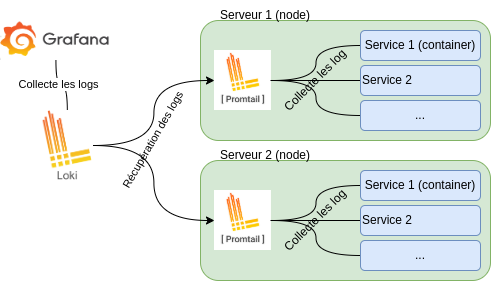
\includegraphics[scale=0.7]{./ressource/loki_Protmail.png}
\end{center}


\section{Pré-requis}
Pour effectuer le test de logs dans les meilleurs conditions, il est nécessaire de stopper les containers des tests précédents. Pour cela, soit vous allez dans \textbf{tous les répertoires} contenant vos \verb?docker-compsoe.yml? et vous taper la commande 
\begin{lstlisting}[style=commande]
sudo docker compose down
\end{lstlisting}

Soit vous taper juste suivante/ Elle arrête tous les containers \textbf{Attention si vous en avez d'autres qui ne doivent pas être arrêtes}.
\begin{lstlisting}[style=commande]
sudo docker stop $(sudo docker ps -q)
\end{lstlisting}

Normalement la commande pour visualiser les container lancés ne retourne rien

\begin{lstlisting}[style=commande]
$ sudo docker ps
CONTAINER ID   IMAGE     COMMAND   CREATED   STATUS    PORTS     NAMES
\end{lstlisting}


\paragraph{Service à scruter} \

Pour les tests, les logs des \textbf{services LEMP en HTTP} (non sécurisé) vont être collectés. Il est donc ncéessaire de le relancer. 
Pour rappel : 
\begin{itemize}
\itemE L'URL du dépôt est  : \url{git@github.com:PierreViland/00-serveurLemp.git}
\itemE La branche a utilisé est : \verb?main?
\begin{lstlisting}[style=commande]
$ git switch main
Already on 'main'
Your branch is up to date with 'origin/main'.
\end{lstlisting}

\itemE La commande pour l'ensemble l'ensemble des containers est : 
\begin{lstlisting}[style=commande]
$ sudo docker compose up -d
\end{lstlisting}


\end{itemize} 

\section{Mise en palce de Promtail}

\end{document}